\newpage
\section{Playing with Blocks}\label{A:B1}
\index{base-ten blocks} 

I always enjoyed blocks quite a bit. Go find yourself
some \textit{base-ten blocks}. Just so that we are all on the same
page, here are the basic blocks:
\[
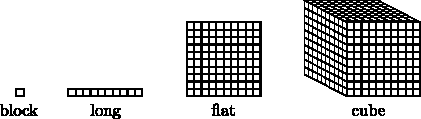
\includegraphics{../graphics/baseTenBlocks.pdf}
\]

\begin{prob} 
Sketch a model of the number $247$ with base-ten blocks.
\vspace{0.8in}
\end{prob}

\begin{prob}
Oscar modeled the number $15$ in the following way:
\[
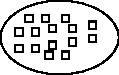
\includegraphics{../graphics/oscarModel.pdf}
\]
What do you think of his model?  Can you improve upon it?  
\vspace{0.5in}
\end{prob}

\begin{teachingnote}
The issue here is that the place-value system is not modeled. When
working with base-ten blocks, we will demand that the place value
system is always modeled.  We want to do this with all algorithms.  
\end{teachingnote}

\begin{prob}
Many problems involving subtraction can be considered one of the following types:  take-away, comparison, and missing addend.  Write a ``word problem'' illustrating each of these types.  
\end{prob}

\newpage

\begin{prob} 
Here is a standard subtraction algorithm:\index{subtraction algorithm!standard}
\[
\begin{tabular}{@{}r@{}r@{}r@{}r@{}}
&   & 8 &  \\
& 8 & $\not{\hspace{-.2ex}9}$ & $\hspace{.3ex}\leftexp{1}2$\\
$-$ & 3 & 7 & 8\\ \hline
& 5 & 1 & 4
\end{tabular}
\]
Use base-ten blocks to model this algorithm.  Which type of subtraction are you using?  
\end{prob}

\newpage
\fixnote{Maybe do the next problem before the previous.}
\begin{prob}
Oscar uses base-ten blocks to model subtraction.  
\[
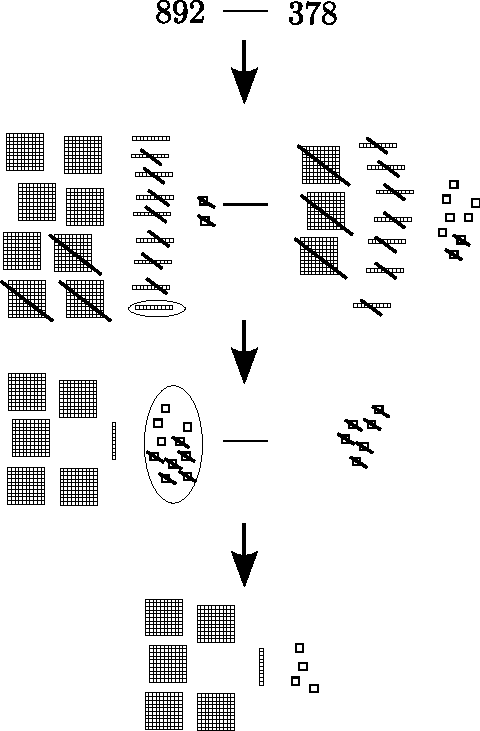
\includegraphics{../graphics/oscarSub.pdf}
\]
Can you explain what is going on?  Which type of subtraction is Oscar using?  
\end{prob}

\begin{prob} Create a ``new'' subtraction algorithm based on Oscar's model.
\end{prob}

\newpage
\begin{prob}
Here is an example of a standard addition algorithm:
\[
\begin{tabular}{@{}r@{}}
11~~\\
892\\
+398\\ \hline
1290
\end{tabular}
\]
Model this algorithm with base-ten blocks.
\end{prob}




